% This is a model template for the solutions in computational science. You can find a very useful documentation for LaTeX in Finnish at ftp://ftp.funet.fi/pub/TeX/CTAN/info/lshort/finnish/ or in English at ftp://ftp.funet.fi/pub/TeX/CTAN/info/lshort/english/. The section List of mathematical symbols in Chapter 3 is especially useful for the typesetting of mathematical formulas.

% Compile the document to PDF by command 'pdflatex model.tex' in the terminal. The command must be run twice for the references in the text to be correct.

\documentclass[a4paper,11pt]{article}
\usepackage[utf8]{inputenc}
% This includes letters such as � and �
\usepackage[T1]{fontenc}
% Use here 'Finnish' for Finnish hyphenation. You may have to compile the code twice after the change.
\usepackage[english]{babel}
\usepackage{graphicx}
% Some math stuff
\usepackage{amsmath,amsfonts,amssymb,amsbsy,commath,booktabs,hyperref,dirtytalk}
% This is just to include the urls
\usepackage{hyperref,subcaption}
\usepackage[margin=2cm]{geometry}
\setlength{\parindent}{0mm}
\setlength{\parskip}{1.0\baselineskip}

\usepackage{listings}
\usepackage{color}
\usepackage{pdfpages,multicol}

\definecolor{dkgreen}{rgb}{0,0.6,0}
\definecolor{gray}{rgb}{0.5,0.5,0.5}
\definecolor{mauve}{rgb}{0.58,0,0.82}

\lstset{frame=tb,
	language=Python,
	aboveskip=3mm,
	belowskip=3mm,
	showstringspaces=false,
	columns=flexible,
	basicstyle={\tiny\ttfamily},
	numbers=none,
	numberstyle=\tiny\color{gray},
	keywordstyle=\color{blue},
	commentstyle=\color{dkgreen},
	stringstyle=\color{mauve},
	breaklines=true,
	breakatwhitespace=true,
	tabsize=4
}
\setlength{\parskip}{0pt}
\begin{document}
\title{Kah-Vis : Visualizing the effect of 
	Bulk Purchase of Coffee on consumption} % Replace the exercise round number
\author{Kunal Ghosh - 546247 - kunal.ghosh@aalto.fi} % Replace with your name and student number
\maketitle
\begin{multicols}{2}
\section*{The Data}
The Chosen dataset comes from the purchase receipts we collected over the past 6 months. In this report we \textbf{focus only on the subset of the data which records the purchase of coffee}. Each such entry also has a corresponding remark section where the (indicative) number of cups consumed were recorded. NOTE : The number of cups for bulk purchases are taken from the of suggested servings on the pack. We would like to test the \textbf{hypothesis that bulk purchase of coffee results in increase in its consumption}.
\section*{Our visualization approach}
\textbf{Who is the Target audience of this visualization ?}: This visualization is to help show the trend in coffee consumption to the person whose purchase dataset we have collected. 
A few questions the user might want an answer to, from our visualization is about  the magnitude (of Cups of coffee and Expenditure) and overall trends if any exist.
To that effect we have aggregated, by month, the Expenditure on Coffee (in Euros) and the number of cups of coffee purchased (or consumed) and we hope this would highlight monthly trends, if any such trends exist. This grouping should also average out any daily or weekly fluctuations in the trend.
\section*{Munzner Model}
The following Data \ref{1} and Task \ref{2} abstractions are based on the Munzer model described in the course slides.
\subsection*{Data Abstraction}
\begin{itemize}
	\item Data Type
	\begin{itemize}
		Attribute
		\begin{enumerate}
			\item Date of Purchase 
			\item Cups of Coffee Purchased
			\item Expenditure (Euros)
		\end{enumerate} 
	\end{itemize}
	\item Dataset Type : Table
	\item Dataset Availability : Static
	\item Attributes Types : Quantitative
\end{itemize}
\subsection*{Task Abstraction}
Chained sequence of tasks or {Action, Target} Pairs.
\begin{itemize}
	\item \textbf{PRODUCE : Derive - Distribution}
	\begin{itemize}
			\item Group the Tabular data by Month. 
	\end{itemize}
	\item \textbf{SEARCH : Explore - Distribution}
	\item \textbf{QUERY : Identify - Trends}
	\begin{itemize}
		\item Plot the trend lines
	\end{itemize}
\end{itemize}
\subsection*{Visual Encoding}
\begin{itemize}
	\item Marks used : Lines
	\begin{itemize}
		\item As bars to encode \textbf{magnitude}
		\item Interpolated lines to highlight the trend \ref{6}
	\end{itemize}	
	\item Visual Variables
	\begin{itemize}
		\item Position : \textbf{Horizontal Position of bars} : Aided by the month labels on the x axis, position of the bars can effectively portray ordinal data according to Mackinlay’s ranking of visual variables \ref{3}
		\item Size : \textbf{Length} of bars used to encode \textbf{magnitude} is the best available (Position already used to convey the ordinal month data) visual variable to denote Quantitative Data, according to  \textbf{Mackinlay’s ranking} [3].
	\end{itemize}
\end{itemize}
\subsection*{Visual Idiom}
A visual idiom is a combination of marks and visual variables.
\begin{itemize}
	\item We have used \textbf{bar plots} to indicate the \textbf{magnitude} as it aids in comparing values. \ref{4}
	\begin{itemize}
		\item Also Bar plots are suitable because in our case, we have 1 key ( Date ) and 1 quantitative  attribute ( Expense and Cups of Coffee )
	\end{itemize}
	\item We have also used a smoothed (cubic interpolated) \textbf{line plot} as it aids in perceiving \textbf{trends}. \ref{5}
	\begin{itemize}
		\item In this case we used date as the ordered key attribute and the corresponding Expense and Cups of Coffee and the quantitative attribute
	\end{itemize}
\end{itemize}
\section*{Tufte’s Principles}	
We have ensured that the bar plots are proportional to the measured quantities. This follows the principle laid down by Tufte which states \textit{“The representation of numbers, as physically measured on the surface of the graphic itself, should be directly proportional to the numerical quantities represented.”}\\\\
Staying in line with tufte’s principle \textit{“The number of information-carrying (variable) dimensions depicted should not exceed the number of dimensions in the data.”} We use only two visual variables to encode the dimensions of time and magnitude.\\\\
\textbf{Data-ink ratio} is maximized by removing the default gray background of the plots along with the panel grids and added light gray horizontal panel axis. Also the facet bounding boxes are removed.
\section*{Gestalt Laws}
\begin{itemize}
	\item \textbf{Continuity} : The overall Trend is better perceived if the trend line is a smooth curve. \ref{7} 
	\item \textbf{Closure} : We have made use of facets to show Two separate quantities with different units and scales. As suggested in \ref{8} 
	\item \textbf{Connectedness} : horizontal grid lines meet to corresponding facet labels indicating connectedness.
\end{itemize}
\section*{Methods used to analyze the data}
\begin{itemize}
	\item We have first filtered the complete set of purchase records to get only the subset of data we were interested in analyzing.
	\item We then \textbf{order the data} by the date to ensure that we get the true trend.
	\item We also \textbf{group the data} by month, to get the monthly cumulative expense and cups of coffee consumed. This helps in averaging out small variabilities in the data.
	\item Finally instead of drawing a linear trend line we chose to use a \textbf{cubic polynomial trend line} which we thought portrayed the overall trend well without being too jagged.
\end{itemize}
\end{multicols}
\begin{figure*}[h]
	\centering
	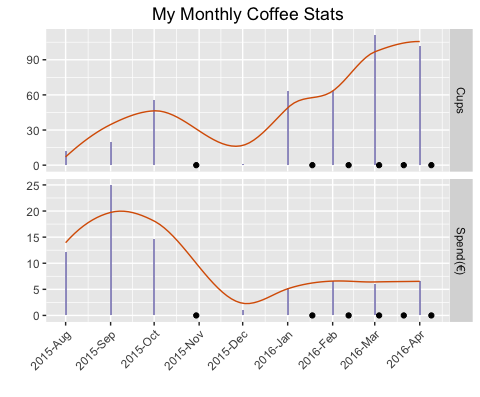
\includegraphics[scale=0.70]{FinalVis.png}
	\caption{The dots correspond to dates when larger packs of Coffee were purchased. \textbf{NOTE}: The consumption is indicative only, if the coffee was purchased on the last day of the month, it would be consumed on the next month. However, it is grouped in the same month in the visualization.
		}
	\label{fig}
\end{figure*}
\begin{multicols}{2}
\section*{Chosen Visualization Technique and Rationale}
In this visualization, We have the challenge of visualizing two quantities (Monthly Expense and Cups of Coffee) it a known problem \ref{8} that having two scales on the vertical axis leaves scope for manipulative visualizations. For example, In case of the trend line, we can change the scales of the graphs to make them intersect. In this case intersection (one plot surpassing the other) does not have any meaning because the units of the two graphs are different.
To avoid the above caveat we make use of facets to show Two separate quantities with different units and scales. It has the advantage of having same Horizontal axis (in this case) which aids in making meaningful comparisons.
Our choice for the bars and line plot is from a color blind and print friendly color palette  as suggested by the ColorBrewer2.org web-application.
\section*{Results}
After analyzing the data and visualizing it, we observe that since the bulk purchase (lower coffee spends) have become more frequent, the consumption has risen steadily and shows a positive trend.
\section*{Discussion on Hypothesis after the results: }
It is quite clear from the graph that bulk purchase (Less monthly expenditure) of coffee definitely corresponds to more consumption. However, we \textbf{cannot yet confirm our Hypothesis based on the above visualization}, it would be more appropriate to draw this conclusion by running this experiment for a few more months and visualize the trends.\\
\vfill
\section*{References}
\begin{enumerate}
	\item T-61-5010 Lecture7 Visualization analysis and design slide 44 \label{1}
	\item T-61-5010 Lecture7 Visualization analysis and design slide 52 \label{2}
	\item T-61-5010 Lecture7 Visualization analysis and design slide 76 \label{3}
	\item T-61-5010 Lecture7 Visualization analysis and design slide 76 \label{4}
	\item T-61-5010 Lecture7 Visualization analysis and design slide 79 \label{5}
	\item Visualization Analysis and Design Page - (Munzner 2015) page 157 \label{6}
	\item T-61-5010 Lecture 6 human perception part3 slide 63 \label{7}
	\item \href{http://www.perceptualedge.com/articles/visual_business_intelligence/dual-scaled_axes.pdf}{Dual-Scaled Axes in Graphs
		Are They Ever the Best Solution? - Stephen Few - 2008} \label{8}
\end{enumerate}
\end{multicols}
\end{document}
